In this chapter, we will discuss a bulk-surface model that is motivated by the interactions of ligands and receptors. We will give a classical proof of existence and uniqueness of weak solutions to this model, as well as discuss some of the qualitative properties of such solutions. The proof will rely heavily on the definitions and results introduced in \autoref{ch:Preliminaries}, and will we based on an application of the Banach fixed-point theorem.

\section{Biological motivation}
\todo{actual biological terms}

Consider an open and bounded set $U \subseteq \R^d$ with $C^1$ boundary and $T > 0$. This can be interpreted as the microscopic part of the body we are investigating. We identify the cells in this part of the body by an open set $C \subseteq U$, also with $C^1$ boundary, and the extracellular space by $\Omega := U \setminus \overline{C}$. We require that the closure $\overline{C}$ of $C$ is also completely contained in $U$, i.e. no cells should touch the boundary of our domain. In particular, this implies that the boundary $\partial \Omega$ of the extracellular space can be written as the disjoint union of the boundary of our region of investigation $\partial U$ and the cell membranes $\partial C$, which we denote by $\Gamma_{e}$ and $\Gamma$, respectively. We use the function $u: [0, T] \times \Gamma \to \R$ to represent the concentration of free receptors at a given time and location on a cell membrane. Similarly, $u_b: [0, T] \times \Gamma \to \R$ represents the concentration of bounded receptors, and $v: [0, T] \times \overline{\Omega} \to \R$ represents the concentration of ligands in $\overline{\Omega}$, see \cref{fig:domain}.

\begin{figure}[!t]
    \centering
    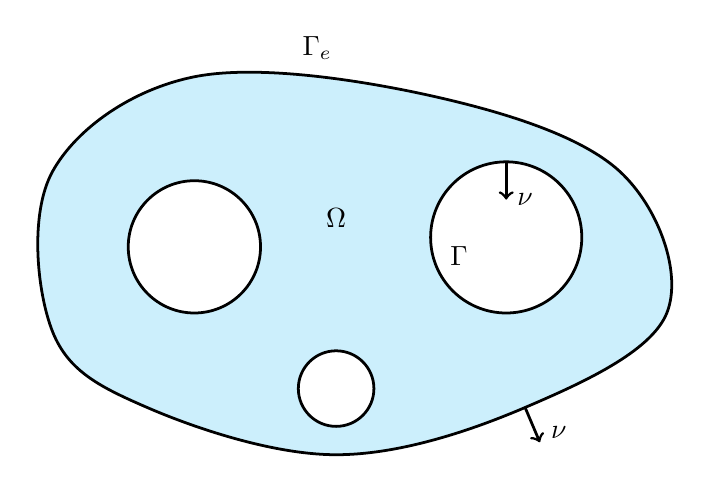
\begin{tikzpicture}[scale=1.2]

    \fill[cyan!20, even odd rule]
    plot[smooth cycle, tension=0.6] coordinates {
        (-3,1.5)
        (-1.5,2.5)
        (1,2.3)
        (3,1.5)
        (3.5,0)
        (2,-1)
        (0,-1.5)
        (-2,-1)
        (-3,-0.2)
    }
    (-1.5,0.7) circle (0.7)
    (1.8,0.8) circle (0.8)
    (0,-0.8) circle (0.4);
    
    % Outer irregular boundary
    \draw[line width=1pt]
      plot[smooth cycle, tension=0.6] coordinates {
        (-3,1.5)
        (-1.5,2.5)
        (1,2.3)
        (3,1.5)
        (3.5,0)
        (2,-1)
        (0,-1.5)
        (-2,-1)
        (-3,-0.2)
      };
    
    % Inner circles
    \draw[line width=1pt] (-1.5,0.7) circle (0.7);
    \draw[line width=1pt] (1.8,0.8) circle (0.8);
    \draw[line width=1pt] (0,-0.8) circle (0.4);
    
    % Labels
    \node at (0.0,1.0) {$\Omega$};
    \node at (1.3,0.6) {$\Gamma$};
    \node at (-0.2,2.8) {$\Gamma_e$};
    \node at (2.0,1.2) {$\nu$};
    \node at (2.356, -1.268) {$\nu$};
    
    % Arrows (boundary directions)
    \draw[->, line width=1pt] (1.8,1.6) -- (1.8,1.2);
    \draw[->, line width=1pt] (2,-1) -- (2.156, -1.368);
    
    \end{tikzpicture}
    \caption{A sketch of a possible domain in the case that $d= 2$. The blue background represents $\Omega$ and the two kinds of boundaries are indicated, along with the outward unit normal vector $\nu$.}
    \label{fig:domain}
\end{figure}

The ligands can move freely through the extracellular space. This can be modelled by the standard diffusion (or heat) equation. To simplify the setting\todo{setting?}, we assume the individual receptors will be fixed in their position on the cell membrane.

When a ligand binds to a free receptor, the concentration of free receptors and ligands decrease, and the concentration of bounded receptors at that position increases accordingly. This reaction is described by $\kon u^2 v$ for some $\kon > 0$. After some time, the bounded receptor has done its task, passing the signal through to the interior of the cell. It releases the ligand and is now available to bind to a new ligand again. The concentration of bounded receptors decrease, and the concentration of free receptors and ligands increase accordingly. The rate of this dissociation is described by $\koff u_b$, where $\koff > 0$.

Finally, two reactions that happen constantly are production and decay. To keep intercellular communication possible, cells produce ligands and receptors that enter the domain $\Omega$ through the cell membrane. We assume the production of ligands and free receptors mainly happens at constant rates $P_u > 0$ and $P_v > 0$, but is also upregulated by the concentration of bounded receptors, which is taken into account by $\alpha u_b$ for some upregulation coefficient $\alpha > 0$. The ligands, free receptors and complex receptors decay at constant rates $\delta_v$, $\delta_u$ and $\delta_{u_b}$, respectively.

We can describe the dynamics of ligands and receptors by a system of coupled differential equations. Denote the diffusion coefficient by $D_v > 0$ and the outward unit normal vector on $\partial \Omega$ by $\nu$. Then the concentrations of receptors can then be described by the system of ODEs given by

\begin{equation}
    \label{sys:ODEs}
    \begin{aligned}
        u_t         &= P_u + \alpha u_b - \delta_u u - 2 \kon u^2 v + 2 \koff u_b   & \text{on }& (0, T) \times \Gamma, \\
        u_{b,t}     &= -\delta_{u_b} u_b + \kon u^2 v - \koff u_b                   & \text{on }& (0, T) \times \Gamma. \\
    \end{aligned}
\end{equation}

\noindent
Note that even though they are given by only two equations, this is actually a system of uncountably many ODEs. For every boundary point $x \in \Gamma$, we have one ODE for the function $t \mapsto u(t, x)$ and one for the function $t \mapsto u_b(t, x)$.

Since the dynamics of the ligands include diffusion in $\Omega$ and reaction on $\Gamma$, they can be described by the PDE and boundary conditions given by

\begin{equation}
    \label{sys:PDEs}
    \begin{aligned}
        v_t                   &= D_v \Delta v - \delta_v v      & \text{in }& (0, T) \times \Omega, \\
        D_v \pderiv[v]{\nu}   &= P_v - \kon u^2 v + \koff u_b   & \text{on }& [0, T) \times \Gamma, \\
        D_v \pderiv[v]{\nu}   &= 0                              & \text{on }& [0, T) \times \Gamma_e. \\
    \end{aligned}
\end{equation}

\noindent
Additionally, we need to specify initial conditions for the concentration of ligands and receptors. That is, the solutions should satisfy

\begin{equation}
    \label{sys:Init}
    \begin{aligned}
        u(0, \cdot\ )          &= u_0           & \text{on }& \Gamma, \\
        u_b(0, \cdot\ )        &= u_{b,0}       & \text{on }& \Gamma, \\
        v(0, \cdot\ )          &= v_0           & \text{on }& \Omega, \\
    \end{aligned}
\end{equation}

\noindent
for some given non-negative functions $u_0, u_{b,0}: \Gamma \to \R$ and $v_0: \Omega \to \R$.

The remainder of this chapter will be dedicated to studying the system of \cref{sys:ODEs,sys:PDEs,sys:Init}.

\section{Weak formulation}
Before we start proving the existence of solutions to this model, we must discuss what kind of solutions we are looking for. Specifically, we will derive the weak formulation of \cref{sys:ODEs,sys:PDEs,sys:Init} and discuss the function spaces that are involved.

As in \cref{sec:weak_forms}, we multiply $v_t$ by a test function $\phi \in C_c^\infty(\Omega)$ and integrate to get

\begin{equation*}
    \begin{aligned}
        \int_\Omega v_t \phi = D \int_\Omega \Delta v \phi &= D \int_{\partial \Omega} \nabla v \cdot \nu \phi \ dS - D \int_\Omega \nabla v \cdot \nabla \phi \\
         &= D \int_{\partial \Gamma} \nabla v \cdot \nu \phi \ dS + D \int_{\partial \Gamma_e} \nabla v \cdot \nu \phi \ dS - D \int_\Omega \nabla v \cdot \nabla \phi \\
         &= - \int_{\partial \Gamma} f(u, u_b, v) \phi \ dS + \int_{\partial \Gamma} r(v) \phi \ dS - D \int_\Omega \nabla v \cdot \nabla \phi, \\
    \end{aligned}
\end{equation*}

\noindent
which we can also write as

\begin{equation}
    \inner{v_t, \phi}_{L^2(\Omega)} = - \inner{f(u, u_b, v), \phi}_{L^2(\Gamma)} + \inner{r(v), \phi}_{L^2(\Gamma)} - D \inner{\nabla v, \nabla \phi}_{L^2(\Omega; \R^d)}.
\end{equation}

\section{Existence and uniqueness}
Our goal in this section is to prove the following theorem.

\begin{theorem}{Existence and uniqueness of weak solutions}{eq_and_un}
    Let the initial conditions $u_0, u_{b, 0} \in \Ltwo{\partial \Omega}$ and $v_0 \in \Ltwo{\Omega}$ be essentially bounded and non-negative. Then there exist unique weak solutions $u, u_b \in H^1(0, T; \Ltwo{\Gamma})$ and $v \in \Ltwo{0, T; H^1(\Omega)}$ with $v_t \in \Ltwo{0, T; H^1(\Omega)^*}$ to \cref{sys:ODEs,sys:PDEs,sys:Init}. Moreover, these solutions are also non-negative and bounded.
\end{theorem}

As previously mentioned, the proof will be based on an application of Banach's fixed-point theorem. The proof for our model follows the same general idea as the proof of the Picard-Lindel\"of theorem proving the existence and uniqueness for ODEs, but we need to adjust the arguments and function spaces to handle our situation of a coupled bulk-surface system. The idea is to consider the problem at a smaller time interval $[0, \widetilde{T}]$ for some $\widetilde{T} \leq T$ and ``freeze'' the function $v$ in the ODEs so we can use the standard existence and uniqueness theory for ODEs to get solutions $u$ and $u_b$ to this problem. The PDE we treat similarly, freezing the functions $u$ and $u_b$. Having a solution of this PDE, we can ``update'' the frozen terms in the ODE. This produces an operator $\mathcal{T}$ that maps any $v \in \pdespace$ to another $\widetilde{v} \in \pdespace$, where $\pdespace$ is the space defined by
%
\begin{equation*}
    \pdespace := \left\{ v \in \Ltwo{0, \widetilde{T}; H^1(\Omega)}\ \middle|\ v_t \in \Ltwo{0, \widetilde{T}; H^1(\Omega)^*} \text{ and } 0 \leq v \leq M_v(T) \text{ almost everywhere} \right\},
\end{equation*}

\noindent
which we view as a closed subset of $\Ltwo{0, \widetilde{T}; \Ltwo{\Omega}}$. We will derive the exact value of $M_v(T)$ later. Defining this operator, we will need another function space $\odespace$ given by
%
\begin{equation*}
    \odespace := \left\{ (u, u_b) \in \left(H^1(0, \widetilde{T}; \Ltwo{\Gamma})\right)^2\ \middle|\ 0 \leq u \leq M_u(T) \text{ and } 0 \leq u_b \leq M_{u_b}(T) \text{ almost everywhere} \right\},
\end{equation*}

\noindent
which we view as a closed subset of the space $(\Ltwo{0, \widetilde{T}; \Ltwo{\Gamma}})^2$. Again, the exact values of $M_u(T)$ and $M_{u_b}(T)$ will be derived later. If we can then show that this operator is a contraction, Banach's fixed-point theorem will guarantee the existence and uniqueness of a fixed point $v^* \in \pdespace$, which will be a local solution to the PDE. We will then show how we can stitch together local solutions to get a unique solution for every final time $T$.

Let us first make precise what we mean by ``freezing'' the function $v$ in the ODE system. Fix $\widetilde{T} \leq T$ and $v^* \in \pdespace$ and consider the modified system of ODEs given by
%
\begin{equation}\label{eq:frozen_odes}
    \begin{aligned}
        u_t         &= P_u + \alpha u_b - \delta_u u - 2 \kon u^2 \gamma v^* + 2 \koff u_b   & \text{on }& (0, \widetilde{T}) \times \Gamma, \\
        u_{b,t}     &= - \delta_{u_b} u_b + \kon u^2 \gamma v^* - \koff u_b                  & \text{on }& (0, \widetilde{T}) \times \Gamma, \\
        u(0)        &= u_0, \qquad u_b(0) = u_{b, 0}                                  & \text{on }& \Gamma. \\
    \end{aligned}
\end{equation}

\noindent
These ODEs are now \emph{decoupled} from the PDE, so we can investigate the existence and uniqueness of solutions to this system without simultaneously having to prove that $v$ is a solution of the PDE.

\begin{lemma}{Existence and uniqueness for the decoupled ODEs}{exun_frozen_odes}
    Let the initial conditions $u_0, u_{b,0} \in \Ltwo{\Gamma}$ be essentially bounded and non-negative and fix $v^* \in \pdespace$. Then there exist unique weak solutions $(u, u_b) \in \odespace$ to \cref{eq:frozen_odes} satisfying these initial conditions.
\end{lemma}

\begingroup
\newcommand{\vb}{\overline{v}}
\newcommand{\vt}{\widetilde{v}}
\newcommand{\ub}{\overline{u}}
\newcommand{\ut}{\widetilde{u}}
\newcommand{\ubb}{\overline{u}_b}
\newcommand{\ubt}{\widetilde{u}_b}
\begin{proof}
    Fix $x$ and define $w$ and $F: \R \times \R^2 \to \R^2$ as in \cref{eq:weak_ode,eq:ode_system_function}, where $v$ is replaced by $v^*$. Since the components of $F$ are polynomial in $w$, the function $F$ is certainly continuous in $w$. Additionally, by the regularity of $\gamma v^*$ which we showed in \cref{prop:trace_regularity}, we know that $F$ is measurable in $t$. This also implies that for any compact subset of $\R \times \R^2$, we can bound $F$ by some time-dependent integrable function $m$. In particular, this subset can be taken to be a rectangle\footnote{On first sight, it can seem strange to call this type of set a rectangle instead of a cylinder. This name comes from the fact that in our main source \cite{coddington_theory_1984}, the theorem is proved for the case of $n = 1$. } as in the hypothesis of \cref{thm:caratheodory}, so let $R$ be such a rectangle around the initial time $t = 0$ and initial data $(u_0, u_{b,0})$. The hypotheses of \cref{thm:caratheodory} are then fully satisfied, giving us a local solution $w: [0, \beta] \to \R^2$ for some $\beta > 0$, with $w(0) = (u_0, u_{b,0})$.

    We show that this local solution is unique. Suppose we have two such local solutions, $w_1$ and $w_2$. Since these solutions are absolutely continuous, they are bounded on $[0, \beta]$, so we can take a compact set $K \subseteq \R^2$ that contains both their trajectories. For any $t \in [0, \beta]$ and $\overline{w} = (\ub, \ubb), \widetilde{w} = (\ut, \ubt) \in K$, $F$ satisfies
%
    \begin{equation*}
    \begin{aligned}
        \left|F(t, \overline{w}) - F(t, \widetilde{w})\right|^2 &= \left| \begin{pmatrix}
            -2 \kon \left(\ub^2 - \ut^2\right) \gamma v^*(t, x) + 2 \koff \left(\ubb - \ubt\right) + \alpha \left(\ubb - \ubt\right) - \delta_u \left(\ub - \ut\right) \\
            \kon \left(\ub^2 - \ut^2\right) \gamma v^*(t, x) - \koff \left(\ubb - \ubt\right) - \delta_{u_b} \left(\ubb - \ubt\right) \\
        \end{pmatrix} \right|^2 \\
        &= \left| \begin{pmatrix}
            - \left(2 \kon \left(\ub + \ut\right) \gamma v^*(t, x) + \delta_u\right) \left(\ub - \ut\right) & + \left(2 \koff + \alpha\right)\left(\ubb - \ubt\right) \\
            \kon \left(\ub + \ut\right) \gamma v^*(t, x) \left(\ub - \ut\right) & - \left(\koff + \delta_{u_b}\right) \left(\ubb - \ubt\right) \\
        \end{pmatrix} \right|^2 \\
        &\leq 2 \left| \begin{pmatrix}
            - 2 \kon \left(\ub + \ut\right) \gamma v^*(t, x) - \delta_u \\
            \kon \left(\ub + \ut\right) \gamma v^*(t, x)
        \end{pmatrix} \left(\ub - \ut\right) \right|^2 + 2 \left| \begin{pmatrix}
            2 \koff + \alpha \\
            \koff + \delta_{u_b}
        \end{pmatrix} \left(\ubb - \ubt\right) \right|^2 \\
        &\leq L_K(t)^2 \left(\left(\ub - \ut\right)^2 + \left(\ubb - \ubt\right)^2\right) \leq L_K(t)^2 \left|\overline{w} - \widetilde{w}\right|^2,
    \end{aligned}
    \end{equation*}

    \noindent
    where $L_K(t)$ is defined as
%
    \begin{equation*}
        L_K(t) := \sqrt{2} \max \left\{ \left| \begin{pmatrix}
            4 \kon \diam(K) v^*(t, x) + \delta_u \\
            2 \kon \diam(K) v^*(t, x)
        \end{pmatrix} \right| ,\quad \left| \begin{pmatrix}
            2 \koff + \alpha \\
            \koff + \delta_{u_b}
        \end{pmatrix} \right| \right\} ,
    \end{equation*}

    \noindent
    which is of $L^2$-regularity in $t$ due to the essential boundedness of $v^*$. Now for the difference of the two solutions we obtain
%
    \begin{equation*}
        \begin{aligned}
            \left|w_1(t) - w_2(t)\right| &= \left|(u_0, u_{b,0}) + \int_{0}^{t} F(t, w_1(t)) \d t - (u_0, u_{b,0}) - \int_{0}^{t} F(t, w_2(t)) \d t \right| \\
            &\leq \int_{0}^{t} \left|F(t, w_1(t)) - F(t, w_2(t))\right| \d t \leq \int_{0}^{t} L_K(t) \left|w_1(t) - w_2(t)\right| \d t
        \end{aligned}
    \end{equation*}

    \noindent
    for every $t \in [0, \beta]$. Using Gronwall's lemma and the fact that $w_1(0) = w_2(0)$, we see that this implies that $\left|w_1(t) - w_2(t)\right| = 0$ for all $t \in [0, \beta]$, so $w_1 = w_2$.

    To show that the components $u$ and $u_b$ of this solution $w$ are non-negative, we multiply the equations of \cref{eq:frozen_odes} by $u_{-} := - \min (0, u)$ and $u_{b, -} := - \min (0, u_b)$, respectively, and obtain
%
    \begin{align*}
        \left( u_{b,-}(t) \right)^2 &= 2 \int_{0}^{t} u_{b,-}(r) \frac{\d}{\d t} u_{b, -}(r)\d r = - 2 \int_{0}^{t} u_{b,-}(r) u_{b, t}(r) \d r \\
        &= - 2 \int_{0}^{t} \left[ - \delta_{u_b} u_b(r) + \kon u(r)^2 \gamma v^*(r, x) - \koff u_b(r) \right] u_{b, -}(r) \d r \\
        &= 2 \int_{0}^{t} \left[ - \delta_{u_b} \left( u_{b,-}(r) \right)^2 - \kon u^2(r) \gamma v^*(r, x) u_{b,-}(r) - \koff \left( u_{b,-}(r) \right)^2 \right] \d r \leq 0,
    \end{align*}

    \noindent
    so $u_{b,-}(t) = 0$ for every $t \in [0, \beta]$, showing that $u_b$ must be non-negative for almost every $t \in [0, \beta]$. Using this in the estimate for $u$, we get
%
    \begin{align*}
        \left( u_{-}(t) \right)^2 &= 2 \int_{0}^{t} u_{-}(r) \frac{\d}{\d t} u_{-}(r)\d r = - 2 \int_{0}^{t} u_{-}(r) u_{t}(r) \d r \\
        &= - 2 \int_{0}^{t} \left[ P_{u} + \alpha u_b(r) - \delta_{u} u(r) - 2 \kon u(r)^2 \gamma v^*(r, x) + 2 \koff u_b(r) \right] u_{-}(r) \d r \\
        &= 4 \kon \int_{0}^{t} u(r)^2 \gamma v^*(r, x)u_{-}(r) \d r \\
        & \qquad - 2 \int_{0}^{t} \left[ P_{u} u_{-}(r) + \alpha u_b(r) u_{-}(r) + \delta_{u} u(r)^2 + 2 \koff u_b(r)u_{-}(r) \right] \d r \\
        &\leq 4 \kon \int_{0}^{t} u(r)^2 \gamma v^*(r, x)u_{-}(r) \d r.
    \end{align*}

    \noindent
    By application of Gronwall's lemma, this shows that $u_-(t) = 0$ for almost all $t \in [0, \beta]$, so $u \geq 0$.
    
    We can use the non-negativity of $u$ and $u_b$ to show that these functions are bounded. Define $r := u + 2 u_b$ and note that
%
    \begin{equation*}
        r_t = u_t + 2 u_{b, t} = P_u - \delta_u u + (\alpha - 2 \delta_{u_b}) u_b \leq P_u + m r,
    \end{equation*}

    \noindent
    where $m := \max\left(\delta_u, \frac{1}{2}(\alpha - 2 \delta_{u_b})\right)$. Then Gronwall's lemma gives
%
    \begin{equation*}
        r(t) \leq e^{mt}\left(r(0) + t P_u\right).
    \end{equation*}

    \noindent
    Now the non-negativity of both $u$ and $u_b$ and the essential boundedness of $u_0$ and $u_{b,0}$ allows us to bound the solutions independent of $\widetilde{T}$ by
%
    \begin{equation}\label{eq:ode_bounds}
    \begin{alignedat}{2}
        u &\leq e^{mT} \left(M + P_u\right) &&=: M_u(T) \qquad \text{and} \\
        u_b &\leq \frac{1}{2} M_u(T) &&=: M_{u_b}(T),
    \end{alignedat}
    \end{equation}

    \noindent
    where $M = \esssup(u_0 + 2 u_{b, 0})$, for almost every $x \in \Gamma$ and $t \in [0, \beta]$.

    Now suppose we have solutions $u$ and $u_b$ on a maximum time interval $[0, \widetilde{\beta})$. Since we have a bound for $u$ and $u_b$ that is independent of $\widetilde{\beta}$, we can use the continuation argument from \cite{coddington_theory_1984} and see that we have a solution for $u$ and $u_b$ on $[0, \widetilde{T}]$.

    Now if we let $x$ vary, we can see that $u$ and $u_b$ are both of $L^2$ regularity in space, because the bounds from \cref{eq:ode_bounds} are independent of space. Lastly, the fact that $u$ and $u_b$ are essentially bounded shows that $u_t$ and $u_{b, t}$ are bounded, so $u, u_b \in H^1(0, \widetilde{T}; \Ltwo{\Gamma})$.
\end{proof}

\endgroup

We can use a similar approach for the PDE in \cref{sys:PDEs}. Fix $(u^*, u_b^*) \in \odespace$ and consider the modified weak formulation given by
%
\begin{equation}\label{eq:frozen_pde}
\begin{split}
    \pair{v_t, \phi} = \inner{P_v, \phi}_{\Ltwo{\Gamma}} - \kon \inner{\left(u^*\right)^2 v, \phi}_{\Ltwo{\Gamma}} + \koff \inner{u_b^*, \phi}_{\Ltwo{\Gamma}} \\
    - D_v \inner{\nabla v, \nabla \phi}_{\Ltwo{\Omega; \R^d}} - \delta_v \inner{v, \phi}_{\Ltwo{\Omega}}.
\end{split}
\end{equation}

\noindent
for almost every $t \in [0, \widetilde{T}]$. This PDE is now decoupled from the ODEs, and we can prove the existence and uniqueness independently from the ODE system.

\begin{lemma}{Existence and uniqueness for the decoupled PDE}{exun_frozen_pde}
    Let the initial condition $v_0 \in \Ltwo{\Omega}$ be essentially bounded and non-negative and fix $(u^*, u_b^*) \in \odespace$. Then there exists a unique weak solution $v \in \pdespace$ to \cref{eq:frozen_pde} satisfying these initial conditions.
\end{lemma}

\begin{proof}
    To prove the existence and uniqueness goes beyond the scope of this thesis. Hence, we assume that a unique weak solution $v$ of the PDE exists and $v$ is essentially bounded by a constant depending on $T$. This can be proven using Galerkin methods, as demonstrated in \cite{evans2010partial}. Let $v$ now be such a solution. To show that $v$ is non-negative, we estimate the negative part of $v$. Let $v_{+}$ and $v_{-}$ be defined as $v_+ := \max(0, v)$ and $v_- := - \min(0, v)$ respectively, such that $v = v_{+} - v_{-}$. Then as discussed in \cite{evans2010partial}, we have $v_{+}, v_{-} \in \Ltwo{0, \widetilde{T}; H^1(\Omega)}$ and $\left(v_{+}\right)_t, \left(v_{-}\right)_t \in \Ltwo{0, \widetilde{T}; H^1(\Omega)^*}$. Furthermore, $v_t v_{-} = - (v_{-})_t v_{-}$, as well as $\nabla v \cdot \nabla v_{-} = - \left|\nabla v_{-}\right|^2$, so for all almost every $t$ we have
%
    \begin{equation*}
         \frac{\d}{\d t} \frac12 \norm{v_{-}}_{\Ltwo{\Omega}}^2 = \pair{(v_-)_t, v_-} = - \pair{v_t, v_{-}}
    \end{equation*}

    \noindent
    due to \cref{thm:lionsmagenes}. We use $v_-$ as a test function and employ the fact that $v$ is a solution to the PDE, which gives
    %
    \begin{equation*}
        \begin{aligned}
         \frac{\d}{\d t} &\frac12 \norm{v_{-}}_{\Ltwo{\Omega}}^2 = - \pair{v_t, v_{-}} = D_v \int_{\Omega} \nabla v \cdot \nabla v_- + \delta_v \int_{\Omega} v v_- - \int_{\Gamma} \left(P_v - \kon u^2 v + \koff u_b\right) v_-  \d S \\
        &= - D_v \norm{\nabla v_-}_{\Ltwo{\Omega; \R^d}}^2 - \delta_v \norm{v_-}_{\Ltwo{\Omega}}^2 - P_v \int_{\Gamma} v_- \d S + \kon \int_{\Gamma} u^2 v v_-  \d S - \koff \int_{\Gamma} u_b v_-  \d S \\
        &= - D_v \norm{\nabla v_-}_{\Ltwo{\Omega; \R^d}}^2 - \delta_v \norm{v_-}_{\Ltwo{\Omega}}^2 - P_v \int_{\Gamma} v_- \d S - \kon \int_{\Gamma} u^2 (v_-)^2  \d S - \koff \int_{\Gamma} u_b v_-  \d S \\
        &\leq 0,
    \end{aligned}
    \end{equation*}

    \noindent
    where we used the non-negativity of $v_-$ and $u_b$ in the last step. By \cref{thm:lionsmagenes}, we know that $v$ is continuous in time with respect to the $L^2$-norm. The only way for this to be achieved while also guaranteeing the time derivative is non-positive, is by having
%
    \begin{equation*}
        \norm{v_{-}}_{\Ltwo{\Omega}} = 0
    \end{equation*}

    \noindent
    for almost every $t$, which implies that $v$ is non-negative.

    % To show boundedness of $v$, we consider $\left( v - M_1 e^{M_2 t} \right)_+$ as a test function for constants $M_1$ and $M_2$. This gives

    % \begin{align*}
    %     \frac{1}{2} \frac{\d}{\d t} \norm{\left( v - M_1 e^{M_2 t} \right)_+}&_{\Ltwo{\Omega}}^2 = \pair{\frac{\d}{\d t} \left( v - M_1 e^{M_2 t} \right)_+, \left( v - M_1 e^{M_2 t} \right)_+} \\
    %     =& \pair{\left( v_t - M_1 M_2 e^{M_2 t} \right), \left( v - M_1 e^{M_2 t} \right)_+} \\
    %     =& \int_\Gamma \left(P_v - \kon \left(u^*\right)^2 v + \koff \left(u_b^*\right)\right) \left( v - M_1 e^{M_2 t} \right)_+ \d S \\
    %      &- \delta_v \int_{\Omega} \left( v - M_1 M_2 e^{M_2 t} \right) \left( v - M_1 e^{M_2 t} \right)_+ \\
    % \end{align*}

    % \todo{Mariya's term?}

    % {\color{red}To show that the map $t \mapsto \norm{v(t)}_{\Ltwo{\Omega}}^2$ is essentially bounded, we use $v$ itself as a test function to get

    % \begin{equation*}
    % \begin{aligned}
    %      \frac{\d}{\d t} \frac12 &\norm{v}_{\Ltwo{\Omega}}^2 = \int_{\Omega} v_t v = \int_{\Gamma} \left(P_v - \kon u^2 v + \koff u_b\right) v \d S - D_v \int_{\Omega} \nabla v \cdot \nabla v - \delta_v \int_{\Omega} v v \\
    %     &= P_v \int_{\Gamma} v \d S - \kon \int_{\Gamma} u^2 v^2 \d S + \koff \int_{\Gamma} u_b v \d S  - D_v \norm{\nabla v}_{\Ltwo{\Omega; \R^d}}^2 - \delta_v \norm{v}_{\Ltwo{\Omega}}^2 \\
    %     &\leq P_v \int_{\Gamma} v \d S + \koff \int_{\Gamma} u_b v \d S - D_v \norm{\nabla v}_{\Ltwo{\Omega; \R^d}}^2 . \\
    % \end{aligned}
    % \end{equation*}

    % \noindent
    % Now we apply Young's equality with $\eps$ to the first two integrals in this last expression to derive   

    % \begin{equation*}
    % \begin{alignedat}{2}
    %     P_v \int_{\Gamma} v \d S &\leq \int_{\Gamma} \left(\eps v^2 + \frac{1}{4 \eps} P_v^2 \right) \d S = \eps \norm{v}_{\Ltwo{\Gamma}}^2 + \frac{1}{4\eps} P_v^2 | \Gamma | &&=: \eps \norm{v}_{\Ltwo{\Omega}}^2 + \frac{1}{2}B_\eps ,\\
    %     \koff \int_\Gamma u_b v &\leq \int_\Gamma \left(\eps + \frac{1}{4 \eps} \koff^2 u_b^2 \right) \d S = \eps \norm{v}_{\Ltwo{\Gamma}}^2 + \frac{1}{4\eps} \koff^2 \norm{w}_{\Ltwo{\Gamma}}^2 &&=: \eps \norm{v}_{\Ltwo{\Gamma}}^2 + \frac{1}{2} D_\eps \norm{w}_{\Ltwo{\Gamma}}^2 ,
    % \end{alignedat}
    % \end{equation*}

    % \noindent
    % which, when plugged into the original estimate, gives

    % \begin{equation*}
    %      \frac{\d}{\d t} \frac12 \norm{v}_{\Ltwo{\Omega}}^2 \leq \frac{1}{2} B_\eps + \frac{1}{2} D_\eps \norm{w}_{\Ltwo{\Gamma}}^2 + 2 \eps \norm{v}_{\Ltwo{\Gamma}}^2 - D_v \norm{\nabla v}_{\Ltwo{\Omega; \R^d}}^2 .
    % \end{equation*}

    % \noindent
    % To convert the $\Ltwo{\Gamma}$-norm of $v$ on the right-hand side into an $\Ltwo{\Omega}$-norm, we employ the trace inequality from \cref{thm:trace} and get

    % \begin{equation*}
    % \begin{aligned}
    %      \frac{\d}{\d t} \frac12 \norm{v}_{\Ltwo{\Omega}}^2 &\leq \frac{1}{2} B_\eps + \frac{1}{2} D_\eps \norm{w}_{\Ltwo{\Gamma}}^2 + 2 \eps C_\gamma^2 \norm{v}_{H^1(\Omega)}^2 - D_v \norm{\nabla v}_{\Ltwo{\Omega; \R^d}}^2 \\
    %     &= \frac{1}{2} B_\eps + \frac{1}{2} D_\eps \norm{w}_{\Ltwo{\Gamma}}^2 + 2 \eps C_\gamma^2 \norm{v}_{\Ltwo{\Omega}}^2 + 2 \eps C_\gamma^2 \norm{\nabla v}_{\Ltwo{\Omega; \R^d}}^2 - D_v \norm{\nabla v}_{\Ltwo{\Omega; \R^d}}^2 \\
    %     &\leq \frac{1}{2} B_\eps + \frac{1}{2} D_\eps \norm{w}_{\Ltwo{\Gamma}}^2 + 2 \eps C_\gamma^2 \norm{v}_{\Ltwo{\Omega}}^2 \\
    %     &=: \frac{1}{2} B_\eps + \frac{1}{2} D_\eps \norm{w}_{\Ltwo{\Gamma}}^2 + \frac{1}{2} A_\eps \norm{v}_{\Ltwo{\Omega}}^2
    % \end{aligned}
    % \end{equation*}

    % \noindent
    % for small enough $\eps > 0$ and almost every $t$. We are now ready to use Gronwall's lemma to get the final estimate \todo{gronwall application}

    % \begin{equation*}
    % \begin{aligned}
    %     \norm{v(t)}_{\Ltwo{\Omega}}^2 &\leq \norm{v_0}_{\Ltwo{\Omega}}^2 e^{A_\eps t} + \int_{0}^{t} \left(B_\eps + D_\eps \norm{w(s)}_{\Ltwo{\Gamma}}^2\right) e^{A_\eps (t - s)} \d s \\
    %     &= \norm{v_0}_{\Ltwo{\Omega}}^2 e^{A_\eps t} + \frac{B_\eps}{A_\eps} \left(e^{A_\eps t} - 1\right) + D_\eps \int_{0}^{t} \norm{w(s)}_{\Ltwo{\Gamma}}^2 e^{A_\eps (t - s)} \d s \\
    %     &\leq \norm{v_0}_{\Ltwo{\Omega}}^2 e^{A_\eps t} + \frac{B_\eps}{A_\eps} \left(e^{A_\eps t} - 1\right) + \frac{D_\eps M_{u_b}(T)^2 |\Gamma|}{A_\eps} \left(e^{A_\eps t} - 1\right) \\
    %     &\leq \norm{v_0}_{\Ltwo{\Omega}}^2 e^{A_\eps T} + \frac{B_\eps}{A_\eps} \left(e^{A_\eps T} - 1\right) + \frac{D_\eps M_{u_b}(T)^2 |\Gamma|}{A_\eps} \left(e^{A_\eps T} - 1\right) \\
    %     &=: M_v(T)
    % \end{aligned}
    % \end{equation*}

    % \noindent
    % for almost every $t$, where $M_{u_b}(T)$ was defined in the proof of \cref{lem:exun_frozen_odes}.}
\end{proof}

Using \cref{lem:exun_frozen_odes,lem:exun_frozen_pde}, we can define two operators between $\pdespace$ and $\odespace$. One takes a function $v^* \in \pdespace$ and maps it to the unique solution $(u, u_b) \in \odespace$ of \cref{eq:frozen_odes}. Let us refer to this operator as $\mathcal{T}_{1}: \pdespace \to \odespace$. The other operator, $\mathcal{T}_{2}: \odespace \to \pdespace$, takes two arbitrary functions $(u^*, u_b^*) \in \odespace$ and defines $\mathcal{T}_{2}(u^*, u_b^*)$ as the unique solution $v \in \pdespace$ to \cref{eq:frozen_pde}. Combining these two operators, we define  
%
\begin{equation*}
    \mathcal{T} := \mathcal{T}_{2} \circ \mathcal{T}_{1} : \pdespace \to \pdespace.
\end{equation*}

\noindent
We want to show that this operator has a unique fixed point. If this is the case, we have a functions $v \in \pdespace$ such that $\mathcal{T}(v) = v$, and let $(u, u_b) \in \odespace$ denote $(u, u_b) = \mathcal{T}_{1}(v)$. Given that then $\mathcal{T}_{2}(u, u_b) = v$, by definition this means that $v$ solves \cref{eq:weak_pde} for almost every $t \in (0, \widetilde{T})$, and $w = (u, u_b)$ solves \cref{eq:weak_ode} for almost every $t \in (0, \widetilde{T})$ and $x \in \Gamma$, meaning that $v$, $u$ and $u_b$ are weak solutions of our model on the local time scale $(0, \widetilde{T})$. Conversely, if $v$, $u$ and $u_b$ are weak solutions to the model, then by the uniqueness of solutions in \cref{lem:exun_frozen_odes,lem:exun_frozen_pde}, we must have that $\mathcal{T}_{2}(u, u_b) = v$ and $\mathcal{T}_{1}(v) = (u, u_b)$, and thus $\mathcal{T}(v) = v$.

It should be clear now how we will apply Banach's fixed-point theorem. If we prove that $\mathcal{T}$ is a contraction, we can guarantee the existence of a fixed point and therefore a weak solution. Since every weak solution of the model is also a fixed point, the theorem also grants us uniqueness of such solutions. To prove that $\mathcal{T}$ is a contraction, we first show this for $\mathcal{T}_{2}$ and $\mathcal{T}_{1}$ separately, after which we can easily combine the results.

\begingroup
\newcommand{\vb}{\overline{v}}
\newcommand{\vt}{\widetilde{v}}
\newcommand{\ub}{\overline{u}}
\newcommand{\ut}{\widetilde{u}}
\newcommand{\ubb}{\overline{u}_b}
\newcommand{\ubt}{\widetilde{u}_b}

\begin{lemma}{}{contraction_pde}
    For $\widetilde{T} > 0$ small enough, $\mathcal{T}_{2}: \odespace \to \pdespace$ is a contraction. That is, there is a $q \in [0, 1)$ such that
    %
    \begin{equation*}
        \norm{\mathcal{T}_{2} (\ub, \ubb) - \mathcal{T}_{2} (\ut, \ubt)}_{\Ltwo{0, \widetilde{T}; \Ltwo{\Omega}}}^2 \leq q \norm{(\ub, \ubb) - (\ut, \ubt)}_{\left(\Ltwo{0, \widetilde{T}; \Ltwo{\Gamma}}\right)^2}^2
    \end{equation*}

    for every $(\ub, \ubb), (\ut, \ubt) \in \odespace$.
\end{lemma}

\begin{proof}
    Let $(\ub, \ubb), (\ut, \ubt) \in \odespace$ and define $\vb, \vt \in \pdespace$ by $\vb := \mathcal{T}_{2}(\ub, \ubb)$ and $\vt := \mathcal{T}_{2}(\ut, \ubt)$. We now denote their differences by
%
    \begin{equation*}
        v := \vb - \vt, \qquad u := \ub - \ut \qquad \text{and} \qquad u_b := \ubb - \ubt,
    \end{equation*}

    \noindent
    such that
%
    \begin{equation*} 
        \norm{\mathcal{T}_{2} (\ub, \ubb) - \mathcal{T}_{2} (\ut, \ubt)}_{\Ltwo{0, \widetilde{T}; \Ltwo{\Omega}}}^2 = \norm{\vb - \vt}_{\Ltwo{0, \widetilde{T}; \Ltwo{\Omega}}}^2 = \norm{v}_{\Ltwo{0, \widetilde{T}; \Ltwo{\Omega}}}^2.
    \end{equation*}

    \noindent
    We can estimate this norm using the weak form of the PDE. We use \cref{thm:lionsmagenes} to see that
%
    \begin{equation*}
    \begin{aligned}
        \frac{\d}{\d t} \frac{1}{2} \norm{v}_{\Ltwo{\Omega}}^2 = \pair{v_t, v} = - D_v \int_\Omega \left|\nabla v\right|^2 - \delta_v \int_\Omega v^2 + \int_\Gamma \left(- \kon \ub^2 \vb + \koff \ubb + \kon \ut^2 \vt - \koff \ubt\right) v \d S ,
    \end{aligned}
    \end{equation*}

    \noindent
    which after rearranging becomes
%
    \begin{equation*}
    \begin{aligned}
        \frac{\d}{\d t} \frac{1}{2} \norm{v}_{\Ltwo{\Omega}}^2 + D_v \norm{\nabla v}_{\Ltwo{\Omega; \R^d}}^2 + \delta_v \norm{v}_{\Ltwo{\Omega}}^2 &= - \kon \int_\Gamma \left(\ub^2 \vb - \ut^2 \vt\right)v \d S + \koff \int_\Gamma u_b v \d S
    \end{aligned}
    \end{equation*}

    \noindent
    for almost all $t$. We then use the identity
%
    \begin{equation} \label{eq:contraction_identity_1}
        \ub^2 \vb - \ut^2 \vt = \ub^2 \vb - \ut^2 \vb + \ut^2 \vb - \ut^2 \vt = (\ub^2 - \ut^2) \vb + \ut^2 v = (\ub + \ut) \vb u + \ut^2 v
    \end{equation}

    \noindent
    to estimate
%
    \begin{equation*}
    \begin{aligned}
        \frac{\d}{\d t} \frac{1}{2} \norm{v}_{\Ltwo{\Omega}}^2 + &D_v \norm{\nabla v}_{\Ltwo{\Omega; \R^d}}^2 + \delta_v \norm{v}_{\Ltwo{\Omega}}^2 \\
        &= - \kon \int_\Gamma \left(\ub + \ut\right) \vb u v \d S - \kon \int_\Gamma \ut^2 v^2 \d S + \koff \int_\Gamma u_b v \d S \\
        &\leq \kon \int_\Gamma \left|(\ub + \ut) \vb u v\right| \d S + \koff \int_\Gamma u_b v \d S \\
        &\leq 2 \kon M_{u}(T) M_v(T) \int_\Gamma \left|u v\right| \d S + \koff \int_\Gamma u_b v \d S .\\
    \end{aligned}
    \end{equation*}

    \noindent
    The mixed terms can be separated using Young's inequality, giving
%
    \begingroup
    \allowdisplaybreaks
    \begin{align*}
        \frac{\d}{\d t} \frac{1}{2} &\norm{v}_{\Ltwo{\Omega}}^2 + D_v \norm{\nabla v}_{\Ltwo{\Omega; \R^d}}^2 + \delta_v \norm{v}_{\Ltwo{\Omega}}^2 \\
        &\leq 2 \kon M_{u}(T) M_v(T) \left(A_{\eps} \norm{u}_{\Ltwo{\Gamma}}^2 + \eps \norm{v}_{\Ltwo{\Gamma}}^2\right) + \koff \left(A_{\eps} \norm{u_b}_{\Ltwo{\Gamma}}^2 + \eps \norm{v}_{\Ltwo{\Gamma}}^2\right) \\
        &\leq B_\eps(T) \norm{u}_{\Ltwo{\Gamma}}^2 + \koff A_{\eps} \norm{u_b}_{\Ltwo{\Gamma}}^2 + C(T) \eps \norm{v}_{\Ltwo{\Gamma}}^2 \\
        &\leq B_\eps(T) \norm{u}_{\Ltwo{\Gamma}}^2 + \koff A_{\eps} \norm{u_b}_{\Ltwo{\Gamma}}^2 + C_\gamma^2 C(T) \eps \norm{v}_{H^1(\Omega)}^2\\
    \end{align*}
    \endgroup

    \noindent
    for almost all $t$. Now let $\delta := \min (\delta_v, D_v)$ and integrate from 0 to $\widetilde{T}$ to get
%
    \begin{equation*}
        \frac{1}{2} \norm{v(t)}_{\Ltwo{\Omega}}^2 + (\delta - C_\gamma^2 C(T) \eps) \norm{v}_{\Ltwo{0, \widetilde{T}; H^1(\Omega)}}^2 \leq B_\eps(T) \norm{u}_{\Ltwo{0, \widetilde{T}; \Ltwo{\Gamma}}}^2 + \koff A_{\eps} \norm{u_b}_{\Ltwo{0, \widetilde{T}; \Ltwo{\Gamma}}}^2
    \end{equation*}

    \noindent
    for almost all $t$. If we now choose $\eps < \frac{\delta}{C_\gamma^2 C(T)}$, we can estimate both the $\Ltwo{0, \widetilde{T}; H^1(\Omega)}$-norm and the $\Ltwo{0, \widetilde{T}; \Ltwo{\Omega}}$-norm of $v$. The first will only be helpful later, but the latter concludes this proof. First, since $\delta - C_\gamma^2 C(T) \eps > 0$, we have
%
    \begin{equation}\label{eq:extra_estimate}
    \begin{aligned}
        \norm{v}_{\Ltwo{0, \widetilde{T}; H^1(\Omega)}}^2 \leq D_\eps(T) \left(\norm{u}_{\Ltwo{0, \widetilde{T}; \Ltwo{\Gamma}}}^2 + \norm{u_b}_{\Ltwo{0, \widetilde{T}; \Ltwo{\Gamma}}}^2\right) .
    \end{aligned}
    \end{equation}

    \noindent
    Second, we can integrate from 0 to $\widetilde{T}$ once more to get
%
    \begin{equation*}
        \norm{v}_{\Ltwo{0, \widetilde{T}; \Ltwo{\Omega}}}^2 \leq \widetilde{T} M_\eps(T) \left(\norm{u}_{\Ltwo{0, \widetilde{T}; \Ltwo{\Gamma}}}^2 + \norm{u_b}_{\Ltwo{0, \widetilde{T}; \Ltwo{\Gamma}}}^2\right).
    \end{equation*}

    \noindent
    Now for $\widetilde{T} < \frac{1}{M_\eps(T)}$, this coefficient is less than 1, so $\mathcal{T}_2$ will be a contraction.
\end{proof}

\begin{lemma}{}{contraction_odes}
    For $\widetilde{T} > 0$ small enough, $\mathcal{T}_{1}: \pdespace \to \odespace$ is a contraction. That is, there is a $q \in [0, 1)$ such that
    %
    \begin{equation*}
        \norm{\mathcal{T}_{1} (\vb) - \mathcal{T}_{1} (\vt)}_{\left(\Ltwo{0, \widetilde{T}; \Ltwo{\Gamma}}\right)^2}^2 \leq q \norm{\vb - \vt}_{\Ltwo{0, \widetilde{T}; \Ltwo{\Omega}}}^2
    \end{equation*}

    for every $\vb, \vt \in \pdespace$.
\end{lemma}

\begin{proof}
    Now let $\vb, \vt \in \pdespace$ and define $\ub, \ubb, \ut$ and $\ubt$ by $(\ub, \ubb) := \mathcal{T}_{1}(\vb)$ and $(\ut, \ubt) := \mathcal{T}_{1}(\vt)$. Once again, we denote their differences by
%
    \begin{equation*}
        v := \vb - \vt, \qquad u := \ub - \ut \qquad \text{and} \qquad u_b := \ubb - \ubt,
    \end{equation*}

    \noindent
    such that
%
    \begin{align*}
        \norm{\mathcal{T}_{1} (\vb) - \mathcal{T}_{1} (\vt)}_{\left(\Ltwo{0, \widetilde{T}; \Ltwo{\Gamma}}\right)^2}^2 &= \norm{(\ub, \ubb) - (\ut, \ubt)}_{\left(\Ltwo{0, \widetilde{T}; \Ltwo{\Gamma}}\right)^2}^2 = \norm{(u, u_b)}_{\left(\Ltwo{0, \widetilde{T}; \Ltwo{\Gamma}}\right)^2}^2 \\
        &= \norm{u}_{\Ltwo{0, \widetilde{T}; \Ltwo{\Gamma}}}^2 + \norm{u_b}_{\Ltwo{0, \widetilde{T}; \Ltwo{\Gamma}}}^2.
    \end{align*}

    \noindent
    We therefore seek to estimate these separate differences $u$ and $u_b$ in terms of $v$. Starting off with $u$, we see that it satisfies
    \begin{equation*}
    \begin{aligned}
        \frac{\d}{\d t} \norm{u}_{\Ltwo{\Gamma}}^2 &= 2 \int_\Gamma u_t u \d S = 2 \int_\Gamma (\ub_t - \ut_t) u \d S \\
        &= 2 \int_\Gamma \left( \alpha (\ubb - \ubt) - \delta_u (\ub - \ut) - 2 \kon (\ub^2 \vb - \ut^2 \vt) + 2 \koff (\ubb - \ubt) \right) u \d S \\
        &= 2 (\alpha + 2 \koff) \int_\Gamma u u_b \d S - 2 \delta_u \int_\Gamma u^2 \d S - 4 \kon \int_\Gamma (\ub^2 \vb - \ut^2 \vt) u \d S
    \end{aligned}
    \end{equation*}

    \noindent
    for almost every $t$. Here, the first step is justified because we know that $u$ belongs to $H^1(0, \widetilde{T}; \Ltwo{\Gamma})$. As we did in the proof of \cref{lem:contraction_pde}, we now use the identity in \cref{eq:contraction_identity_1} to conclude that
    %
    \begin{equation*}
    \begin{aligned}
        \frac{\d}{\d t} \norm{u}_{\Ltwo{\Gamma}}^2 &= 2 (\alpha + 2 \koff) \int_\Gamma u u_b \d S - 2 \delta_u \int_\Gamma u^2 \d S - \overbrace{4 \kon \int_\Gamma (\ub + \ut) \vb u^2 \d S }^{\geq 0} - 4 \kon \int_\Gamma \ut^2 v u \d S \\
        &\leq 2 (\alpha + 2 \koff) \int_\Gamma u u_b \d S - 2 \delta_u \int_\Gamma u^2 \d S + 4 \kon \int_\Gamma \ut^2 \left| v u \right| \d S \\
        &\leq 2(\alpha + 2 \koff) \int_\Gamma u u_b \d S - 2 \delta_u \norm{u}_{\Ltwo{\Gamma}}^2 + 4 \kon M_u (T)^2 \int_\Gamma | v u | \d S . \\
    \end{aligned}
    \end{equation*}
    
    \noindent
    To further separate the mixed terms, we use Young's inequality twice and obtain the estimate
%
    \begin{equation*}
    \begin{aligned}
        \frac{\d}{\d t} \norm{u}_{\Ltwo{\Gamma}}^2 &\leq A_1(T) \norm{u}_{\Ltwo{\Gamma}}^2 + A_2 \norm{u_b}_{\Ltwo{\Gamma}}^2 + \widetilde{B_1}(T) \norm{v}_{\Ltwo{\Gamma}}^2 , \\
        &\leq A_1(T) \norm{u}_{\Ltwo{\Gamma}}^2 + A_2 \norm{u_b}_{\Ltwo{\Gamma}}^2 + B_1(T) \norm{v}_{H^1(\Omega)}^2 , \\
    \end{aligned}
    \end{equation*}

    \noindent
    where $A_1(T)$, $A_2$, $\widetilde{B_1}(T)$ and $B_1(T)$ are defined as
%
    \begin{equation*}
        \begin{aligned}
            A_1(T) &:= - 2 \delta_u + \alpha + 2 \koff + 2 \kon M_u (T)^2 ,& A_2 &:= \alpha + 2 \koff \\
            \widetilde{B_1}(T) &:= 2 \kon M_u (T)^2 \qquad \text{and} & B_1(T) &:= C_\gamma^2 \widetilde{B_1}(T) .
        \end{aligned}
    \end{equation*}

    \noindent
    Using the same arguments, we get a similar estimate for $\frac{\d}{\d t} \norm{u_b}_{\Ltwo{\Gamma}}^2$, namely

    \begingroup
    \allowdisplaybreaks
    \begin{align*}
        \frac{\d}{\d t} \norm{u_b}_{\Ltwo{\Gamma}}^2 &= 2 \int_\Gamma \left(\left(\ubb\right)_t - \left(\ubt\right)_t\right) u_b \d S \\
        &= - 2 \left(\delta_{u_b} + \koff\right) \int_\Gamma u_b^2 \d S + 2 \kon \int_\Gamma \left(\ub^2 \vb - \ut^2 \vt\right) u_b \d S \\
        &= - 2 \left(\delta_{u_b} + \koff\right) \int_\Gamma u_b^2 \d S + 2 \kon \int_\Gamma \left(\ub + \ut\right) \vt u u_b \d S + 2 \kon \int_\Gamma \ut^2 v u_b \d S \\
        &\leq - 2 \left(\delta_{u_b} + \koff\right) \int_\Gamma u_b^2 \d S + 2 \kon \int_\Gamma \left(\ub + \ut\right) \vt \left| u u_b \right| \d S + 2 \kon \int_\Gamma \ut^2 \left| v u_b \right| \d S \\
        &\leq - 2 \left(\delta_{u_b} + \koff\right) \int_\Gamma u_b^2 \d S + 4 \kon M_u(T) M_v(T) \int_\Gamma \left| u u_b \right| \d S + 2 \kon M_u(T)^2 \int_\Gamma \left| v u_b \right| \d S \\
        &\leq A_3(T) \norm{u_b}_{\Ltwo{\Gamma}}^2 + A_4(T) \norm{u}_{\Ltwo{\Gamma}}^2 + \widetilde{B_2}(T) \norm{v}_{\Ltwo{\Gamma}}^2 ,\\
        &\leq A_3(T) \norm{u_b}_{\Ltwo{\Gamma}}^2 + A_4(T) \norm{u}_{\Ltwo{\Gamma}}^2 + B_2(T) \norm{v}_{H^1(\Omega)}^2 ,\\
    \end{align*}
    \endgroup

    \noindent
    where $A_3(T)$, $A_4(T)$, $\widetilde{B_2}(T)$ and $B_2(T)$ are given by
%
    \begin{equation*}
        A_3(T) := 2 \kon M_u(T) M_v(T) + \kon M_u(T)^2 - 2 \delta_{u_b} - 2 \koff ,
    \end{equation*}
    \begin{equation*}
        A_4(T) := 2 \kon M_u(T) M_v(T), \qquad \widetilde{B_2}(T) := \kon M_u(T)^2  \qquad \text{and} \qquad B_2(T) := C_\gamma^2 \widetilde{B_2}(T) .
    \end{equation*}
    
    \noindent
    To combine these estimates, we set
    %
    \begin{equation*}
        A(T) := 2 \max \left(A_1(T), A_2, A_3(T), A_4(T)\right) \qquad \text{and} \qquad B(T) := 2 \max \left(B_1(T), B_2(T)\right)
    \end{equation*}

    \noindent
    and sum them to get
%
    \begin{equation*}
        \frac{\d}{\d t} \left(\norm{u}_{\Ltwo{\Gamma}}^2 + \norm{u_b}_{\Ltwo{\Gamma}}^2\right) \leq A(T) \left(\norm{u}_{\Ltwo{\Gamma}}^2 + \norm{u_b}_{\Ltwo{\Gamma}}^2\right) + B(T) \norm{v}_{H^1(\Omega)}^2
    \end{equation*}

    \noindent
    for almost all $t$. An application of Gronwall's lemma gives
    %
    \begin{equation*}
    \begin{aligned}
        \norm{u(t)}_{\Ltwo{\Gamma}}^2 + \norm{u_b(t)}_{\Ltwo{\Gamma}}^2 &\leq e^{t A(T)} \left[ \norm{u(0)}_{\Ltwo{\Gamma}}^2 + \norm{u_b(0)}_{\Ltwo{\Gamma}}^2 + B(T) \int_{0}^{t} \norm{v(s)}_{H^1(\Omega)}^2 \d s \right] \\
        &\leq B(T) e^{T A(T)} \norm{v}_{\Ltwo{0, \widetilde{T}; H^1(\Omega)}}^2 , \\
    \end{aligned}
    \end{equation*}

    \noindent
    since the initial conditions of $\ub$ and $\ut$ are the same, and therefore $u(0) = 0$ for every $x \in \Gamma$. Naturally, the same holds for $u_b(0)$. After integrating from 0 to $\widetilde{T}$, we can conclude that
%
    \begin{equation*}
        \norm{u}_{\Ltwo{0, \widetilde{T}; \Ltwo{\Gamma}}}^2 + \norm{u_b}_{\Ltwo{0, \widetilde{T}; \Ltwo{\Gamma}}}^2 \leq \widetilde{T} B(T) e^{T A(T)} \norm{v}_{\Ltwo{0, \widetilde{T}; H^1(\Omega)}}^2 .
    \end{equation*}

    \noindent
    It may seem like we are done now, but the current estimate uses the wrong norm on $v$. To get an estimate using the $\Ltwo{0, \widetilde{T}; \Ltwo{\Omega}}$-norm instead, we can use \cref{eq:extra_estimate} to get

    \begin{multline}
        \norm{u}_{\Ltwo{0, \widetilde{T}; \Ltwo{\Gamma}}}^2 + \norm{u_b}_{\Ltwo{0, \widetilde{T}; \Ltwo{\Gamma}}}^2 \\
        \leq \widetilde{T} B(T) e^{T A(T)} D_\eps(T) \left(\norm{u}_{\Ltwo{0, \widetilde{T}; \Ltwo{\Gamma}}}^2 + \norm{u_b}_{\Ltwo{0, \widetilde{T}; \Ltwo{\Gamma}}}^2\right) + \overbrace{\widetilde{T} B(T) e^{T A(T)} \norm{v}_{\Ltwo{0, \widetilde{T}; \Ltwo{\Omega}}}^2}^{\geq 0},
    \end{multline}

    \noindent
    or after rearranging terms,
%
    \begin{equation*}
    \begin{aligned}
        \norm{u}_{\Ltwo{0, \widetilde{T}; \Ltwo{\Gamma}}}^2 + \norm{u_b}_{\Ltwo{0, \widetilde{T}; \Ltwo{\Gamma}}}^2 \leq \frac{\widetilde{T} B(T) e^{T A(T)}}{1 - \widetilde{T} B(T) e^{T A(T)} D_\eps(T)} \norm{v}_{\Ltwo{0, \widetilde{T}; \Ltwo{\Omega}}}^2.
    \end{aligned}
    \end{equation*}

    \noindent
    As this factor clearly approaches 0 when $\widetilde{T}$ goes to 0, we can choose $\widetilde{T}$ sufficiently small such that it is less than 1 and conclude the proof.
\end{proof}

We have now gathered the needed auxiliary results to prove the main statement of this section.

\begin{proof}[Proof of \cref{thm:eq_and_un}]
    Let $\widetilde{T} > 0$ be small enough such that, by \cref{lem:contraction_pde,lem:contraction_odes}, $\mathcal{T}_1$ and $\mathcal{T}_2$ are contractions with Lipschitz constants $q_1$ and $q_2$, respectively. Define, as discussed before, $\mathcal{T}$ as the composition of $\mathcal{T}_1$ and $\mathcal{T}_2$. Then for any $\vb, \vt \in \Ltwo{0, \widetilde{T}; \Ltwo{\Omega}}$, we have
%
    \begin{equation*}
        \norm{\mathcal{T}(\vb) - \mathcal{T}(\vt)}_{\Ltwo{0, \widetilde{T}; \Ltwo{\Omega}}}^2 \leq q_2 \norm{\mathcal{T}_1(\vb) - \mathcal{T}_1(\vt)}_{\left(\Ltwo{0, \widetilde{T}; \Ltwo{\Gamma}}\right)^2}^2 \leq q_2 q_1 \norm{\vb - \vt}_{\Ltwo{0, \widetilde{T}; \Ltwo{\Omega}}}^2 ,
    \end{equation*}

    \noindent
    showing that $\mathcal{T}$ is a contraction since $q_2 q_1 \in [0, 1)$. We apply Banach's fixed-point theorem to get a unique fixed point $v \in \Ltwo{0, \widetilde{T}; \Ltwo{\Omega}}$. As previously discussed, this corresponds to a unique weak solution on $(0, \widetilde{T})$. 
    
    We now seek to extend this to a solution on $(0, T)$. Since all bounds for $u$, $u_b$ and $v$ were derived independently of $\widetilde{T}$, we can set new initial conditions
    %
    \begin{equation*}
        \vt_0 := v(\tfrac12 \widetilde{T}) \qquad \text{and} \qquad(\ut_0, \widetilde{u}_{b,0}) = (u(\tfrac12 \widetilde{T}), u_b(\tfrac12 \widetilde{T})) := \mathcal{T}_1(v)(\tfrac12 \widetilde{T})
    \end{equation*}
    
    \noindent
    and get the same contraction estimates. This gives another local solution $\vt$, this time defined on $(\frac12 \widetilde{T}, \frac32 \widetilde{T})$. Because of the uniqueness properties of both $v$ and $\vt$, their overlap on $(\frac12 \widetilde{T}, \widetilde{T})$ must coincide. This means that $\vt$ can be used to define an extension of $v$ to the interval $(0, \frac32 \widetilde{T})$.

    This process can be repeated, getting a solution on $(\frac{j}{2} \widetilde{T}, \frac{j + 2}{2} \widetilde{T})$ for $j = 2, \dots$ and using them to define extensions of $v$ until we cover the full time interval $(0, T)$. We can simultaneously construct the corresponding solutions to the ODEs by extending the local solutions using $(\ut, \ubt) := \mathcal{T}_1(\vt)$ at every step. For these solutions $u$, $u_b$ and $v$, the same non-negativity and boundedness properties hold as for all the local solutions, since these properties were proven independently of $\widetilde{T}$.
\end{proof}

\endgroup

% \begin{enumerate}
%     \item For every $v^* \in \mathcal{X}$, define $\mathcal{T}_{2} (v^*)$ as the solution $(u^*, u_b^*) \in \mathcal{Y}^2$ to the ODEs~\ref{temp:ode} with frozen reactions.
%     \item For every $(u^*, u_b^*) \in \mathcal{Y}^2$, define $\mathcal{T}_{1} (u^*, u_b^*)$ as the solution $v^* \in \mathcal{X}$ of the PDE~\ref{temp:pde} with frozen flux.
% \end{enumerate}

% We want to use the Picard-Lindel\"of theorem to prove existence and uniqueness of the ODEs. If we fix a solution of the PDEs $v$, we have a system

% \begin{equation}
%     \label{temp:ode}
%     \begin{aligned}
%         \partial_t u(t,x)    &= f(t, x, u(t,x), u_b(t,x)), \\
%         \partial_t u_b(t,x)  &= g(t, x, u(t,x), u_b(t,x)), \\
%     \end{aligned}
% \end{equation}

% \noindent
% where $f$ and $g$ both depend on the trace $v$. We need $f$ and $g$ to be Lipschitz continuous in $u$ and $u_b$ and continuous in time. The former follows from the definition of the model(???), but for the latter, we need continuity of $v$ on $\partial C$. In other words, for every $x \in \partial C$, we need the function $t \mapsto v \vert_{\partial C}(t, x)$ to be continuous. Then for every $x$, we can solve the system~\ref{temp:ode} for $u(\ \cdot\ , x)$ and $u_b(\ \cdot\ , x)$. What can we say about $u(t,\ \cdot\ )$ and $u_b(t,\ \cdot\ )$?

% For fixed $u$ and $u_b$, we have the following equations for $v$:

% \begin{equation}
%     \label{temp:pde}
%     \begin{aligned}
%         v_t(t, x) &= D\Delta v(t, x) && \text{on } (0, T) \times E,\\
%         D \pderiv[v]{\nu}(t, x) &= h(t, x, v(t, x)) && \text{on } (0, T) \times \partial C,\\
%         D \pderiv[v]{\nu}(t, x) &= 0 && \text{on } (0, T) \times \partial C,\\
%     \end{aligned}
% \end{equation}

% \noindent
% where $h$ depends on $u$ and $u_b$.

% \begin{equation*}
%     \begin{aligned}
%         \mathcal{X} &:= \left\{ v \in \Ltwo{0, T; \Omega} \cap C([0, T]; \Ltwo{\Omega}) \mid v \geq 0 \text{ and } v \vert_{\partial C}(\ \cdot\ , x) \in C([0, T]) \text{ for every } x \in \partial C \right\} \\
%         \mathcal{Y} &:= \left\{ u \in \Ltwo{0, T; H^1(\Omega)} \mid u \geq 0 \text{ and } u' \in \Ltwo{0, T; H^{-1}(\Omega)} \right\}
%     \end{aligned}
% \end{equation*}

% \noindent
% Questions:

% \begin{enumerate}
%     \item ODE is not Lipschitz, only locally?
%     \item Picard Lindel\"of for weak solutions?
%     \item Inward flow theorem for weak solutions?
%     \item When do we have time continuity of the trace?
%     \item System of ODEs $\rightarrow$ What can we say about $u(t,\ \cdot\ )$?
% \end{enumerate}
